\chapter{ATIVIDADES DESENVOLVIDAS}

Este capítulo apresentará a parte técnica de um produto na forma de software, inicialmente por meio de uma \textit{Application Programming Interface (API)}, posteriormente adaptada com um Front-End, como possível solução da problemática em questão. Na sequência, será abordada sobre a organização do sistema, o escopo do projeto, as questões de armazenamento de dados e as tecnologias escolhidas para o desenvolvimento da aplicação. Ademais, o projeto possui apenas fins educacionais e exemplificativos até o presente momento.

\section{Escopo do Projeto}

O projeto tem como objetivo facilitar a busca e divulgação de caronas de forma ágil e organizada, melhorando uma prática já existente na região, mas que atualmente é desorganizada e de alcance limitado. Por meio de uma aplicação, será possível uma comunicação mais eficiente entre os usuários, além de oferecer maior segurança e valores competitivos para todos os envolvidos.


\section{Organização Inicial}

Primordialmente, foi fundamental criar uma organização no\textit{ GitHub} para gerenciar futuras atualizações do projeto entre os desenvolvedores, a qual pode ser acessada por meio do link: [https://github.com/projeto-integrador-tads/].

\subsection{Requisitos Funcionais}

Na sequência, foi realizado o levantamento dos requisitos técnicos, divididos em funcionais e não funcionais, com o objetivo de identificar os recursos mínimos necessários para o funcionamento inicial da aplicação, bem como visualizar possíveis necessidades futuras, visando garantir um melhor desempenho na versão final. Nesse contexto, as funcionalidades foram definidas na ``Tabela 12'' como requisitos funcionais do sistema e, na ``Tabela 13'', como requisitos não funcionais - responsáveis por descrever as possíveis restrições do sistema até o presente momento, podendo ser implementadas futuramente.

%Tabela de levantamentos de requisitos Funcionais 
\begin{longtblr}[,
	caption = {Tabela de Requisitos Funcionais do Sistema.},
	label = {tab:requisitos},
	]{
		width = \linewidth,
		colspec = {Q[140]Q[160]Q[680]},
		row{1} = {c},
		cell{2}{1} = {c},
		cell{2}{2} = {c},
		cell{3}{1} = {c},
		cell{3}{2} = {c},
		cell{4}{1} = {c},
		cell{4}{2} = {c},
		cell{5}{1} = {c},
		cell{5}{2} = {c},
		cell{6}{1} = {c},
		cell{6}{2} = {c},
		cell{7}{1} = {c},
		cell{7}{2} = {c},
		cell{8}{1} = {c},
		cell{8}{2} = {c},
		hlines,
		vlines,
	}
	\textbf{Referência} & \textbf{Requisito} & \textbf{Descrição}\\
	RF01 & Criação de conta & Um novo usuário poderá ser cadastrado informando um nome, e-mail e número de telefone.\\
	RF02 & Cadastro de veículo & Cadastrar um veículo é o que possibilitará ao usuário oferecer uma carona.\\
	RF03 & Reserva de carona & Os usuários podem solicitar ou oferecer uma carona. A segunda possibilidade somente será válida para aqueles com algum veículo devidamente registrado na plataforma.\\
	RF04 & Mensagens & Os interessados na carona poderão trocar mensagens entre si com o objetivo de facilitar o encontro, definir horários e decidir detalhes da viagem.\\
	RF05 & Filtrar caronas na região & Todos os usuários podem ver as caronas oferecidas na região especificada. Cada anúncio terá informações de destino, hora da viagem, lugares disponíveis e, se aplicável, o valor.\\
	RF06 & Avaliações & A avaliação ocorrerá entre motorista e passageiro, sendo uma etapa fundamental para garantir a segurança de todos os usuários. Poderá ser atribuída uma mensagem de caráter opinativo para o público e uma nota que varia de 1 a 5.\\
	RF07 & Serviços de e-mail & Envio de e-mails específicos de notificação após determinadas ações do usuário. Será possível disparar mensagens de boas vindas, criação de corrida bem sucedida, desativação e reativação de conta, entre outras.
\end{longtblr}

% Tabela requisitos não funcionais 
% \usepackage{tabularray}
\begin{longtblr}[,
	caption = {Requisitos Não Funcionais do Sistema.},
	label = {tab:requisitos},
	]{
		width = \linewidth,
		colspec = {Q[140]Q[160]Q[680]},
		row{1} = {c},
		cell{2}{1} = {c},
		cell{2}{2} = {c},
		cell{3}{1} = {c},
		cell{3}{2} = {c},
		cell{4}{1} = {c},
		cell{4}{2} = {c},
		cell{5}{1} = {c},
		cell{5}{2} = {c},
		cell{6}{1} = {c},
		cell{6}{2} = {c},
		cell{7}{1} = {c},
		cell{7}{2} = {c},
		cell{8}{1} = {c},
		cell{8}{2} = {c},
		hlines,
		vlines,
	}
	\textbf{Referência} & \textbf{Requisito} & \textbf{Descrição}\\
	RNF01 & Verificação de documentos pessoais~ & Validar se os documentos cadastrados na plataforma são válidos.\\
	RNF02 & Consulta veicular & Consultar se os dados do veículo informados pelo usuário estão cadastrados na base de dados do departamento de trânsito.\\
	RNF03 & Pesquisa de antecedentes criminais & A funcionalidade poderia aumentar a segurança do usuário.\\
	RNF04 & Ranking de confiança & Os usuários com a melhor pontuação poderiam ter privilégios de divulgação ao oferecer ou solicitar uma carona.\\
	RNF05 & Pagamentos & Serviços de pagamento com o objetivo de monetizar a aplicação, além da possibilidade de motoristas lucrarem de forma justa.~\\
	RNF06 & Mensagens automatizadas & O usuário pode utilizar um recurso de inteligência artificial para gerar mensagens rápidas no chat ao solicitar ou oferecer uma carona.\\
	RNF07 & Canal de Suporte & Canal dedicado para oferecer suporte para possíveis problemas e esclarecer dúvidas frequentes.
	
\end{longtblr}



% INICIO Critérios de Aceitação
\subsection{Critérios de Aceitação}

Os Critérios de Aceitação são utilizados para garantir que o software atenda aos requisitos estabelecidos e ofereça uma experiência segura e funcional aos usuários. Esta seção define as condições e requisitos que devem ser cumpridos para que a versão final do sistema seja considerada aprovada e esteja pronta para uso.

\begin{enumerate}
	
	\item \textbf{Cadastro de Usuários}
	\begin{itemize}
		\item Usuários devem se cadastrar com e-mail válido e senha forte.
		\item O e-mail deve ser único.
		\item A senha deve ter no mínimo 8 caracteres.
		\item Usuários devem fornecer informações pessoais básicas.
		
	\end{itemize}
	
	\item \textbf{Segurança}
	
	\begin{itemize}
		\item Encriptação de senha no banco de dados com um\textit{ hash}.
		\item As fotos de perfil e documentos ficarão salvos na \textit{Amazon S3} seguindo as normas da LGPD.
		\item E-mails de alerta quando dados críticos sofrerem alteração (e-mail, senha).
		\item Alterar a senha possui uma quantidade máxima de tentativas por \textit{token}.
	\end{itemize}
	
	\item \textbf{Perfil de Usuário}
	
	\begin{itemize}
		\item Usuários podem atualizar seu perfil a qualquer momento.
		\item Possibilidade de alterar nome, telefone, foto de perfil, etc.
		\item Endereço de e-mail e data de nascimento não podem ser alterados sem verificação adicional.
		\item Usuários devem verificar seu e-mail após o cadastro.
		\item Envio de um e-mail de confirmação com um link para ativar a conta.
	\end{itemize}
	
	\item \textbf{Cadastro de Veículos}
	
	\begin{itemize}
		\item Motoristas devem cadastrar seus veículos para oferecer caronas.
		\item Informar marca, modelo, ano, placa, cor e número de assentos disponíveis.
		\item Motoristas devem enviar documentos comprobatórios relativos ao veículo.
	\end{itemize}
	
	\item \textbf{Publicação de Viagens}
	
	\begin{itemize}
		\item Motoristas podem criar viagens detalhando rota, data, hora e pontos de embarque/desembarque.
		\item Especificar preço por passageiro, se aplicável.
		\item Informar restrições ou preferências dos envolvidos na viagem.
		\item As viagens devem ser criadas com antecedência mínima.
		\item Definir um tempo mínimo antes do horário de partida para criação de novas viagens.
	\end{itemize}
	
	\item \textbf{Reserva de Caronas}
	
	\begin{itemize}
		\item Passageiros podem reservar vagas nas viagens disponíveis.
		\item Confirmar a reserva mediante pagamento, se aplicável.
		\item Notificação para motorista e passageiro sobre a reserva confirmada.
		\item Passageiros podem cancelar suas reservas.
		\item Definir, quando aplicável, políticas de cancelamento e reembolso.
	\end{itemize}
	
	\item \textbf{Avaliação e Feedback}
	
	\begin{itemize}
		\item Usuários podem avaliar e deixar feedback sobre as viagens.
		\item Motoristas e passageiros podem se avaliar mutuamente.
		\item Avaliações devem ser visíveis nos perfis dos usuários.
	\end{itemize}
	
	\item \textbf{Suporte}
	
	\begin{itemize}
		\item Monitoramento e resolução de problemas.
		\item Canal de suporte ao usuário para resolução de problemas e disputas.
	\end{itemize}
	
\end{enumerate}

\section{Back-end}

Para alcançar o objetivo do trabalho, foi desenvolvida uma API que permitirá futuras adaptações para um aplicativo mobile. Essa API será responsável pelo gerenciamento do cadastro e autenticação dos usuários, permitindo que eles solicitem e divulguem caronas na região. Além disso, incluirá a funcionalidade de avaliação dos usuários com base no histórico de viagens, garantindo maior segurança.

\subsection{Arquitetura do \textit{Back-end}}

Durante a produção de qualquer software é necessário garantir que o sistema seja robusto, eficiente e adaptável às necessidades do usuário. Com essa finalidade existe a arquitetura de sistema, responsável pela estrutura e organização dos componentes de um software, incluindo a maneira como esses elementos interagem entre si e com o ambiente externo. Com a finalidade de seguir os padrões de mercado, definiu-se um conjunto de regras para o \textit{Back-end} aplicando os saberes adquiridos nas matérias de Programação Orientada a Objetos, Programação Web I e Banco de Dados I. A \textit{API} em questão trabalha com o estilo \textit{REST} para comunicação entre os componentes, além de separar as responsabilidades da aplicação em três partes principais, conhecidas como \textit{Model, View e Controller}. A estrutura de pastas pode ser observada na Figura 1:
% figura 1
\begin{figure}[h]
	\centering
	\caption{Estrutura de Pastas do Projeto.}
	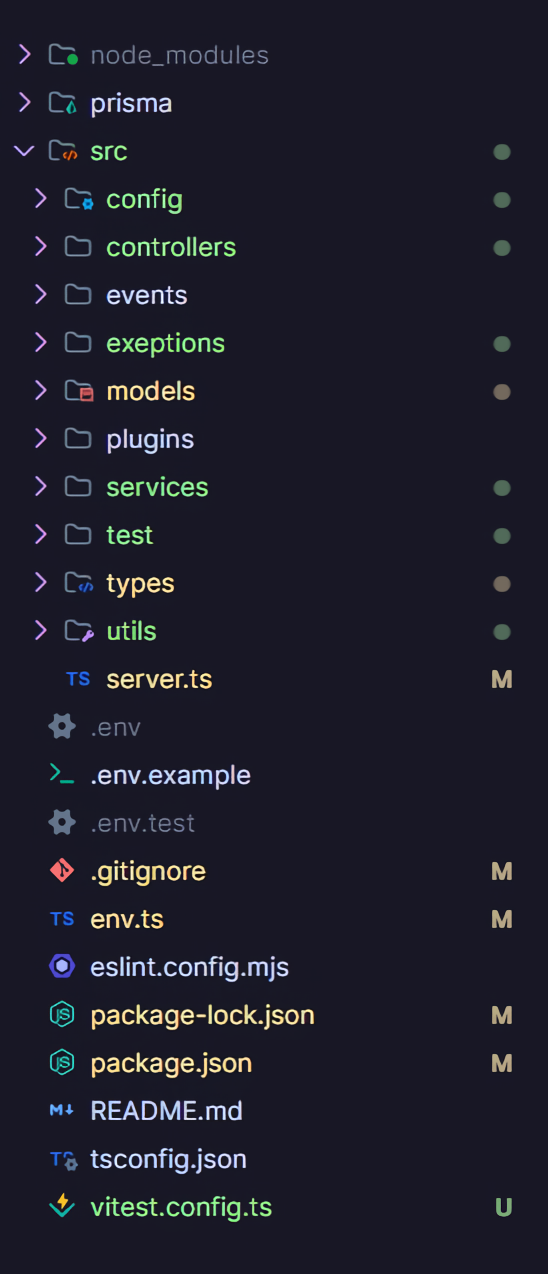
\includegraphics[scale=0.23]{img/pastas.png}
	\legend{Fonte: Autoria Própria}
	\label{fig:EstruturaDePastas}
\end{figure}



% INICIO banco de dados
\subsection{Banco de Dados}

A construção de um banco de dados foi necessário para fazer testes de requisição na \textit{API} desenvolvida. Neste contexto, serão introduzidos o Diagrama Entidade-Relacionamento (DER) e o Modelo Entidade-Relacionamento (MER), para representar graficamente a organização das entidades e os vínculos entre os dados no sistema. Em seguida, serão descritos o esquema do banco de dados, suas tabelas e os relacionamentos estabelecidos entre elas. Essas representações visuais ajudam na compreensão da estrutura lógica e física do banco de dados, bem como facilita o processo de manutenção e expansão futura do software.

\subsection{Diagrama Entidade-Relacionamento (MER)}

A construção deste diagrama conceitual foi de suma importância para a modelagem de dados, representando o mini mundo em questão de um possível aplicativo de caronas. Transformar um recorte do mundo real, para o significado dos dados e como eles se relacionam colaboram na precisão das buscas de informações armazenadas no servidor. O \textit{``Anexo A''} mostra o diagrama entidade-relacionamento deste projeto.


\subsection{Modelo Entidade-Relacionamento (DER)}

Após a modelagem do diagrama anterior, foi possível utilizar o BrModelo para realizar a conversão das tabelas necessárias no banco de dados. O DER facilita a compreensão do MER, tornando a estrutura do banco de dados mais intuitiva e visual, detalhando as chaves primárias, estrangeiras e as cardinalidades. O \textit{``Anexo B''} apresenta as tabelas convertidas, suas chaves e cardinalidades.

\subsection{Dicionário de Dados}

O Dicionário de Dados é uma utilizada em projetos acadêmicos e de desenvolvimento de software, pois descreve detalhadamente as tabelas que compõem o banco de dados relacional, bem como seus atributos. Esta seção tem como objetivo proporcionar uma visão clara e organizada da estrutura do banco de dados, listando as entidades e suas respectivas características. No contexto deste trabalho, as principais tabelas incluem Usuários, Endereços, Motoristas, Veículos, Viagens, Reservas, Mensagens e Avaliações. As tabelas de 1 a 11 apresentam as descrições de cada tabela do banco, incluindo suas principais colunas e uma breve explicação dos atributos mais relevantes.

% tabela de usuário
\begin{longtblr}[
	caption = {Descrição da Entidade Usuários. },
	label = {tab:requisitos},
	entry = none,
	]{
		width = \linewidth,
		colspec = {Q[190]Q[160]Q[620]},
		row{1} = {c},
		row{2} = {c},
		cell{1}{1} = {c=3}{0.938\linewidth},
		cell{3}{1} = {c},
		cell{3}{2} = {c},
		cell{4}{1} = {c},
		cell{4}{2} = {c},
		cell{5}{1} = {c},
		cell{5}{2} = {c},
		cell{6}{1} = {c},
		cell{6}{2} = {c},
		cell{7}{1} = {c},
		cell{7}{2} = {c},
		cell{8}{1} = {c},
		cell{8}{2} = {c},
		cell{9}{1} = {c},
		cell{9}{2} = {c},
		cell{10}{1} = {c},
		cell{10}{2} = {c},
		cell{11}{1} = {c},
		cell{11}{2} = {c},
		cell{12}{1} = {c},
		cell{12}{2} = {c},
		cell{13}{1} = {c},
		cell{13}{2} = {c},
		cell{14}{1} = {c},
		cell{14}{2} = {c},
		cell{15}{1} = {c},
		cell{15}{2} = {c},
		cell{16}{1} = {c},
		cell{16}{2} = {c},
		cell{17}{1} = {c},
		cell{17}{2} = {c},
		hlines,
		vlines,
	}
	\textbf{Usuários}                &                         &                  \\
	\textbf{NOME}                    & \textbf{TIPO DE DADOS}  & \textbf{DESCRIÇÃO}\\
	
	{(PK)\\id\_usuario} 			 & VARCHAR                 & Chave primaria Identificador único da tabela ``usuarios''.\\
	
	nome                             & VARCHAR                 & Nome do usuário.\\
	
	{segundo\_nome}                  & VARCHAR                 & Sobrenome do usuário.\\
	
	email                            & VARCHAR~                & E-mail único, utilizado para login.\\
	
	senha                            & VARCHAR~                & {Senha forte, com no mínimo 8 caracteres, incluindo\\letras maiusculas, minúsculas, números e caracteres\\especiais.} \\
	
	telefone                         & VARCHAR                 & Número de telefone válido.\\
	
	foto\_perfil                     & VARCHAR~                & Caminho para a foto de perfil do usuário.\\
	
	eh\_motorista                    & BOOLEAN                 & Diferencia o usuário do motorista.\\
	
	ativo                            & BOOLEAN                 & Salva a informação se o usuário é ativo.\\
	
	{classificacao\\\_media}         & DOUBLE                  & Nota média do usuário.\\
	
	data\_criacao                    & DATE                    & Armazena a data da criação do perfil.\\
	
	data\_atualizacao                & DATE                    & Ultima atualização do usuário.
	
\end{longtblr}



% Tabela TOKEN
\begin{longtblr}[
	caption = {Descrição da Entidade Token.},
	label = {tab:requisitos},
	entry = none,
	]{
		width = \linewidth,
		colspec = {Q[190]Q[160]Q[620]},
		row{1} = {c},
		row{2} = {c},
		cell{1}{1} = {c=3}{0.938\linewidth},
		cell{3}{1} = {c},
		cell{3}{2} = {c},
		cell{4}{1} = {c},
		cell{4}{2} = {c},
		cell{5}{1} = {c},
		cell{5}{2} = {c},
		cell{6}{1} = {c},
		cell{6}{2} = {c},
		cell{7}{1} = {c},
		cell{7}{2} = {c},
		cell{8}{1} = {c},
		cell{8}{2} = {c},
		hlines,
		vlines,
	}
	
	\textbf{Token}        &                        &                                               \\
	
	\textbf{NOME}         & \textbf{TIPO DE DADOS} &  \textbf{DESCRIÇÃO}\\
	
	{(PK)\\id\_token}	  &     VARCHAR            &  Chave primária, identificador único da tabela ``token''. ~\\
	  
	token      			  &     VARCHAR            &  Armazena o token único gerado para a solicitação de recuperação de senha. \\
	
	{expiracao\_em} 	  &     DATETIME           &  Armazena a data e hora em que o token expira.~\\
	
	{(FK)\_usuarios}	  &     VARCHAR   	       &  Chave estrangeira, referência à tabela ``usuarios''.
	
\end{longtblr}


% Tabela Mensagens
\begin{longtblr}[
	caption = {Descrição da Entidade Mensagens.},
	label = {tab:requisitos},
	entry = none,
	]{
		width = \linewidth,
		colspec = {Q[190]Q[160]Q[620]},
		row{1} = {c},
		row{2} = {c},
		cell{1}{1} = {c=3}{0.941\linewidth},
		cell{3}{1} = {c},
		cell{3}{2} = {c},
		cell{4}{1} = {c},
		cell{4}{2} = {c},
		cell{5}{1} = {c},
		cell{5}{2} = {c},
		hlines,
		vlines,
	}
	\textbf{MENSAGENS}    &                        &                                                \\
	\textbf{NOME}         & \textbf{TIPO DE DADOS} & \textbf{DESCRIÇÃO}                              \\
	
	{(PK) \\id\_mensagem} & VARCHAR                & Chave primária, identificador único da mensagem. \\
	
	conteudo              & VARCHAR                & Armazena o conteúdo das mensagens trocadas.       \\
	
	data\_envio           & DATETIME               & Data do envio da mensagem.~                       \\
	
	{(FK)\_remetente}     & VARCHAR                & Chave estrangeira, referência à tabela ``usuarios'', representando o usuário que enviou a mensagem.~  \\
	
	{(FK)\_viagens}       & VARCHAR                & Chave estrangeira, referência à tabela ``viagens''.~            \\
	
	{(FK)\\\_destinatario}  & VARCHAR              & Chave estrangeira, referência à tabela ``usuarios'', representando o usuário que recebeu a mensagem.~
	                     
\end{longtblr}


% Tabela VIAGENS
\begin{longtblr}[
	caption = {Descrição da Entidade Viagens.},
	label = {tab:requisitos},
	entry = none,
	]{
		width = \linewidth,
		colspec = {Q[190]Q[160]Q[620]},
		row{1} = {c},
		row{2} = {c},
		cell{1}{1} = {c=3}{0.94\linewidth},
		cell{3}{1} = {c},
		cell{3}{2} = {c},
		cell{4}{1} = {c},
		cell{4}{2} = {c},
		cell{5}{1} = {c},
		cell{5}{2} = {c},
		cell{6}{1} = {c},
		cell{6}{2} = {c},
		cell{7}{1} = {c},
		cell{7}{2} = {c},
		cell{8}{1} = {c},
		cell{8}{2} = {c},
		cell{9}{1} = {c},
		cell{9}{2} = {c},
		cell{10}{1} = {c},
		cell{10}{2} = {c},
		cell{11}{1} = {c},
		cell{11}{2} = {c},
		cell{12}{1} = {c},
		cell{12}{2} = {c},
		cell{13}{1} = {c},
		cell{13}{2} = {c},
		cell{14}{1} = {c},
		cell{14}{2} = {c},
		cell{15}{1} = {c},
		cell{15}{2} = {c},
		cell{16}{1} = {c},
		cell{16}{2} = {c},
		cell{17}{1} = {c},
		cell{17}{2} = {c},
		hlines,
		vlines,
	}
	\textbf{VIAGENS}            &                         &                   \\
	\textbf{NOME}               & \textbf{TIPO DE DADOS}  & \textbf{DESCRIÇÃO} \\
	
	{(PK) \\id\_viagem}         & VARCHAR                 & Chave primária, identificador da tabela viagem.\\
	
	status                      & ENUM                    & Armazena os possíveis status da corrida, variando entre agendado, em andamento, concluído ou cancelado.\\
	
	{data\_criacao}             & DATETIME                & Data da criação da corrida.~\\
	
	preco                       & DECIMAL                 & Preço da corrida, quando aplicável a monetização da mesma.\\
	
	{hora\_termino}             & DATETIME                & Registra a hora que a corrida acaba.\\
	
	{preferencias}              & VARCHAR                 & Preferências da corrida definidas pelos participantes antes do seu início.\\
	 
	{data\_atualizacao}         & DATETIME                & Data de atualização mais recente da viagem.\\
	
	{hora\_partida}             & DATETIME                & Define a hora de início de uma viagem.\\
	
	{lugares\\\_disponiveis}    & INT                     & Armazena a quantidade de assentos disponíveis para os passageiros, de acordo com o veículo cadastrado pelo motorista.\\

	{(FK)\_motorista}           & VARCHAR                 & Chave estrangeira, referência à tabela ``motoristas''.\\ 
	
	{(FK)\_endereco\\\_destino} & VARCHAR                 & Chave estrangeira, referência à tabela ``enderecos'', representando o endereço de destino da viagem.\\
	
	{(FK)\_endereco\\\_partida} & VARCHAR                 & Chave estrangeira, referência à tabela ``enderecos'', representando o endereço de partida da viagem.\\
	
	{(FK)\_veiculo}             & VARCHAR                 & Chave estrangeira, referência à tabela ``veiculos''.\\

\end{longtblr}


% Tabela RESERVAS
\begin{longtblr}[
	caption = {Descrição da Entidade Reservas.},
	label = {tab:requisitos},
	entry = none,
	]{
		width = \linewidth,
		colspec = {Q[190]Q[160]Q[620]},
		row{1} = {c},
		row{2} = {c},
		cell{1}{1} = {c=3}{0.938\linewidth},
		cell{3}{1} = {c},
		cell{3}{2} = {c},
		cell{4}{1} = {c},
		cell{4}{2} = {c},
		cell{5}{1} = {c},
		cell{5}{2} = {c},
		cell{6}{1} = {c},
		cell{6}{2} = {c},
		cell{7}{1} = {c},
		cell{7}{2} = {c},
		cell{8}{1} = {c},
		cell{8}{2} = {c},
		hlines,
		vlines,
	}
	\textbf{RESERVAS}      &                        & \\
	\textbf{NOME}          & \textbf{TIPO DE DADOS} & \textbf{DESCRIÇÃO}\\
	
	{(PK)\\id\_reserva}    & VARCHAR                & Chave primária, identificador único da tabela ``reservas''.\\
	
	{data\_criacao}        & DATETIME               & Armazena a data da criação no momento em que a reserva é feita.~\\
	
	{data\_atualizacao}    & DATETIME               & Armazena a data em que a viagem foi atualizada.             \\
	 
	status                 & ENUM                   & Armazena os possíveis status da reserva, variando entre agendado, em andamento, concluído ou cancelado.\\
	
	{status\\\_pagamento}  & ENUM                   & Armazena os possíveis status de pagamento quando aplicável. \\
	
	{(FK)\_passageiro}     & VARCHAR                & Chave estrangeira, referência à tabela ``usuarios'', representando o usuário que solicita a viagem. ~ \\
	
	{(FK)\_viagens}        & VARCHAR                & Chave estrangeira, referência à tabela ``viagens''. \\
	
	
\end{longtblr}

% Tabela AVALIACOES
\begin{longtblr}[
	caption = {Descrição da Entidade Avaliações.},
	label = {tab:requisitos},
	entry = none,
	]{
		width = \linewidth,
		colspec = {Q[190]Q[160]Q[620]},
		row{1} = {c},
		row{2} = {c},
		cell{1}{1} = {c=3}{0.939\linewidth},
		cell{3}{1} = {c},
		cell{3}{2} = {c},
		cell{4}{1} = {c},
		cell{4}{2} = {c},
		cell{5}{1} = {c},
		cell{5}{2} = {c},
		cell{6}{1} = {c},
		cell{6}{2} = {c},
		cell{7}{1} = {c},
		cell{7}{2} = {c},
		cell{8}{1} = {c},
		cell{8}{2} = {c},
		hlines,
		vlines,
	}
	\textbf{AVALIAÇÕES}   &                        &  \\
	\textbf{NOME}         & \textbf{TIPO DE DADOS} & \textbf{DESCRIÇÃO}\\
	
	{(PK)\\id\_avaliacao} & VARCHAR                & Chave primária, identificador único da avaliação.\\
	
	avaliacao             & INT                    & Numeral de 1 a 5 representando a nota da avaliação.\\
	
	comentario            & VARCHAR                & Mensagem de avaliação do usuário.~\\

	{data\_criacao}       & DATETIME               & Data de criação do registro.\\
	
	{data\_atualizacao}   & DATETIME               & Data da modificação mais recente. \\

	{(FK)\_avaliador}     & VARCHAR                & Chave estrangeira, referência à tabela ``usuarios'', representando o usuário que avaliará.   \\
	 
	{(FK)\_viagens}       & VARCHAR                & Chave estrangeira, referência à tabela ``viagens''. \\
	
	{(FK)\_avaliado}      & VARCHAR                & Chave estrangeira, referência à tabela ``usuarios'', representando o usuário que será avaliado.
	
\end{longtblr}


% Tabela ENDEREÇOS
\begin{longtblr}[
	caption = {Descrição da Entidade Endereços.},
	label = {tab:requisitos},
	entry = none,
	]{
		width = \linewidth,
		colspec = {Q[190]Q[160]Q[620]},
		row{1} = {c},
		row{2} = {c},
		cell{1}{1} = {c=3}{0.938\linewidth},
		cell{3}{1} = {c},
		cell{3}{2} = {c},
		cell{4}{1} = {c},
		cell{4}{2} = {c},
		cell{5}{1} = {c},
		cell{5}{2} = {c},
		cell{6}{1} = {c},
		cell{6}{2} = {c},
		cell{7}{1} = {c},
		cell{7}{2} = {c},
		cell{8}{1} = {c},
		cell{8}{2} = {c},
		cell{9}{1} = {c},
		cell{9}{2} = {c},
		hlines,
		vlines,
	}
	\textbf{ENDEREÇOS}        &                        &                           \\
	\textbf{NOME}             & \textbf{TIPO DE DADOS} & \textbf{\textbf{DESCRIÇÃO}}\\
	
	{(PK)\\id\_endereco}      & VARCHAR                & Chave primária, identificador único do endereço.\\
	
	cidade                    & VARCHAR                & Nome da cidade.\\
	
	longitude                 & DOUBLE                 & Coordenada geográfica que especifica a posição norte-sul de uma cidade específica. É de suma importância nas requisições.\\
	
	latitude                  & VARCHAR                & Coordenada geográfica que especifica a posição leste–oeste de uma cidade específica. É de suma importância nas requisições.\\
	
	{endereco\\\_formatado}   & VARCHAR                & Nome formatado do endereço. Importante para a precisão das pesquisas, uma vez que algumas localizações possuem nomes populares, não registrados pelos serviços de geolocalização.\\
	
	ativo                     & BOOLEAN                & Salva a informação se o endereço é ativo.\\
	
	{data\_criacao}           & DATETIME               & Data de criação do registro.\\
	
	{data\_atualizacao}       & DATETIME               & Data da última atualização. \\
	
	{(FK)\_usuarios}          & VARCHAR                & Chave estrangeria, referência a tabela ``usuarios''.
	
\end{longtblr}


% Tabela VEÍCULOS
\begin{longtblr}[
	caption = {Descrição da Entidade Veículos.},
	label = {tab:requisitos},
	entry = none,
	]{
		width = \linewidth,
		colspec = {Q[190]Q[160]Q[620]},
		row{1} = {c},
		row{2} = {c},
		cell{1}{1} = {c=3}{0.941\linewidth},
		cell{3}{1} = {c},
		cell{3}{2} = {c},
		cell{4}{1} = {c},
		cell{4}{2} = {c},
		cell{5}{1} = {c},
		cell{5}{2} = {c},
		cell{6}{1} = {c},
		cell{6}{2} = {c},
		cell{7}{1} = {c},
		cell{7}{2} = {c},
		cell{8}{1} = {c},
		cell{8}{2} = {c},
		cell{9}{1} = {c},
		cell{9}{2} = {c},
		cell{10}{1} = {c},
		cell{10}{2} = {c},
		cell{11}{1} = {c},
		cell{11}{2} = {c},
		cell{12}{1} = {c},
		cell{12}{2} = {c},
		cell{13}{1} = {c},
		cell{13}{2} = {c},
		hlines,
		vlines,
	}
	\textbf{VEÍCULOS}         &                         &                  \\
	\textbf{NOME}             & \textbf{TIPO DE DADOS}  & \textbf{DESCRIÇÃO}\\
	
	{(PK) \\id\_veiculo}      & VARCHAR                 & Chave primária, identificador único do veículo.\\
	
	data\_atualizacao         & DATETIME                & Data da última alteração dos dados do veículo.~\\
	
	cor                       & VARCHAR                 & Cor do veículo.\\
	
	marca                     & VARCHAR                 & Descreve a marca do veículo.\\
	
	data\_criacao             & DATETIME                & Data de cadastro do veículo.\\
	
	ativo                     & BOOLEAN                 & Verifica se o veículo ainda está ativo na aplicação ou não. \\
	
	ano                       & INT                     & Ano de fabricação do veículo.\\
	
	placa                     & VARCHAR                 & Salva o número da placa do veículo após o seu registro.\\ 
	
	capacidade                & INT                     & Quantidade máxima de passageiros que o veículo registrado deve possuir.\\
	
	modelo                    & VARCHAR                 & Descreve o modelo do veículo.~\\
	
	{(FK)\\\_proprietario}    & VARCHAR                 & Chave estrangeira, referência à tabela ``usuarios'', representando o usuário proprietário do veículo.
	
	
\end{longtblr}

%Fim das tabelas 

\subsection{Relacionamentos}

\begin{enumerate}
	
	
	\item \textbf{Usuários - Reservas}
	\begin{itemize}
		\item (1,N): Um usuário pode fazer várias reservas.
		\item (1,1): Cada reserva é feita por um único usuário.
	\end{itemize}
	
	\item \textbf{Usuários - Avaliações}
	\begin{itemize}
		\item (1,N): Um usuário pode fazer várias avaliações.
		\item (1,1): Cada avaliação é feita por um único usuário.
	\end{itemize}	
	
		\item \textbf{Usuários - Mensagens}
	\begin{itemize}
		\item (1,N): Um usuário pode enviar e receber várias mensagens.
		\item (1,1): Cada mensagem tem um remetente e um destinatário únicos, podendo envolver diferentes usuários.
	\end{itemize}
	
		\item \textbf{Usuários - Endereços}
	\begin{itemize}
		\item (1,N): Um usuário pode ter vários endereços.
		\item (1,1): Cada endereço pertence a um único usuário.
	\end{itemize}
	
		\item \textbf{Usuários - Token}
	\begin{itemize}
		\item (1,N): Um usuário pode ter vários TokenJwtExpirado.
		\item (1,1): Cada TokenJwtExpirado pertence a um único usuário.
	\end{itemize}
	
	\item \textbf{Motoristas - Veículos}
	\begin{itemize}
		\item (1,N): Um motorista pode ter vários veículos.
		\item (1,1): Cada veículo está associado a um único motorista
	\end{itemize}
	
	\item \textbf{Motoristas - Viagens}
	\begin{itemize}
		\item (1,N): Um motorista pode criar várias viagens.
		\item (1,1): Cada viagem é conduzida por um único motorista.
	\end{itemize}
	
	\item \textbf{Viagens - Reservas}
	\begin{itemize}
		\item (1,N): Uma viagem pode ter várias reservas.
		\item (1,1): Cada reserva está associada a uma única viagem.
	\end{itemize}
	
	\item \textbf{Viagens - Avaliações}
	\begin{itemize}
		\item (1,N): Uma viagem pode ter várias avaliações.
		\item (1,1): Cada avaliação é feita para uma única viagem.
	\end{itemize}
	
	\item \textbf{Endereço - Viagens}
	\begin{itemize}
		\item (1,1): Uma viagem tem um endereço associado.
		\item (1,N): Cada endereço pode estar associado a várias viagens.
	\end{itemize}
	
	\item \textbf{Mensagens - Viagens}
	\begin{itemize}
		\item (1,N): Uma viagem pode ter várias mensagens associadas.
		\item (1,1): Cada mensagem pode estar se referir a uma única viagem.
	\end{itemize}
	
	\item \textbf{Veículo - Viagens}
	\begin{itemize}
		\item (1,N): Um veículo pode ser utilizado em várias viagens.
		\item (1,1): Cada viagem utiliza um único veículo.
	\end{itemize}
\end{enumerate}

\section{Front-end}

O desenvolvimento do front-end do aplicativo VemComigo foi orientado para proporcionar uma experiência intuitiva e acessível aos usuários. As escolhas durante esta etapa seguem os conhecimentos adquiridos nas aulas de Banco de Dados II, Análise e Projeto de Sistemas, Práticas Profissionais Integradoras II e Desenvolvimento Web II.

\subsection{Arquitetura do Front-End}

Primeiramente, foi realizada a prototipação das possíveis telas com o auxílio de um projeto criado no Figma, o qual pode ser acessado por meio do link:[https://abrir.link/PMhoA]. Criou-se pastas no projeto com a finalidade de melhor organizar as projeções do visual da aplicação. Os primeiros esboços visuais da aplicação encontram-se na página ``Wireframes''. O desing de alta fidelidade foi projetado na sequência e pode ser encontrado na página ``Desing'' do projeto. Por fim, para integrar a API do back-end desenvolvida anteriormente ao front-end, escolheu-se o React Native como framework do JavaScript, visando a criação de uma aplicação multiplataforma eficiente e de forma paralela para Android e IOS. Foi necessário utilizar o Expo como uma ferramenta auxiliar nos testes das telas desenvolvidas, garantindo que os componentes estivessem bem posicionados na tela.

\subsection{Design e UX (Experiência do Usuário)}

A interface foi projetada com foco na responsividade, usabilidade e experiência do usuário, permitindo que esses, mesmo que em diferentes dispositivos móveis, tenham uma utilização intuitiva e fluida. O VemComigo é uma aplicação voltada para a mobilidade e deslocamento de pessoas, dito isso, imagina-se que o usuário final busca simplicidade para escolher rapidamente um meio viável de transporte em meio a agitação do dia a dia. Nesse contexto, decidiu-se então que as telas deveriam ser minimalistas de forma que apenas informações necessárias ocupassem espaço na tela, evitando confusões em usuários mais desatentos. A ``tabela \ref{tab:design-ux}'' apresenta as escolhas que compõem o padrão visual da aplicação.

\begin{longtblr}[
	caption = {Design e UX (Experiência do Usuário)},
	label = {tab:design-ux},
	entry = none,
	]{
		width = \linewidth,
		colspec = {Q[170,c]Q[620]},
		row{1} = {c},
		row{2} = {c},
		cell{1}{1} = {c=2}{0.941\linewidth},
		cell{3}{1} = {c},
		cell{3}{2} = {c},
		cell{4}{1} = {c},
		cell{4}{2} = {c},
		cell{5}{1} = {c},
		cell{5}{2} = {c},
		cell{6}{1} = {c},
		cell{6}{2} = {c},
		cell{7}{1} = {c},
		cell{7}{2} = {c},
		hlines,
		vlines,
	}
	\textbf{Design e UX (Experiência do Usuário)} &  \\
	
	\textbf{Aspecto} & \textbf{Descrição} \\
	
	\textbf{Tipografia} & A fonte escolhida para o aplicativo foi a Poppins, uma tipografia moderna e elegante, amplamente utilizada em interfaces digitais por sua excelente legibilidade em diferentes tamanhos de tela. O uso de diferentes pesos (light, regular, semibold e bold) permitiu hierarquizar informações e destacar conteúdos importantes sem comprometer a estética da interface. \\
	
	\textbf{Paleta de Cores} & Cor principal: \#0064D2 (Azul vibrante) – representa confiança, tecnologia e mobilidade.  
	Cor de Fundo: \#FFFFFF (Branco) – proporciona um ambiente limpo e moderno, facilitando a leitura e destacando os elementos interativos. Cores secundárias e de apoio: tons de cinza e azul escuro foram utilizados para equilibrar a interface e manter um visual neutro e sofisticado. \\
	
	\textbf{Componentes Visuais} & A biblioteca de componentes ``Tamagui'' foi utilizada para melhorar os aspectos visuais e garantir a otimização da aplicação. Adotou-se também uma biblioteca de ícones chamada ``Tabler'', disponível em [https://tabler.io/admin-template]. \\
	
	\textbf{Inputs e Formulários} & Os campos de entrada (inputs) foram projetados para serem acessíveis e de fácil identificação. Foram aplicados bordas arredondadas, espaçamento adequado e feedback visual para indicar erros ou sucessos nas interações dos usuários. Os botões seguem um estilo minimalista, utilizando o azul primário (\#0064D2) para submeter ações principais. \\
	
	\textbf{Logo e Identidade Visual} & O logotipo do aplicativo foi desenvolvido para refletir o conceito de transporte de maneira abstrata. Utilizou-se uma abordagem minimalista, incorporando elementos gráficos que remetem a um formato de uma roda. \\
	
	\textbf{Acessibilidade} & Foram aplicadas boas práticas de acessibilidade, garantindo contraste adequado, tamanhos de fonte ajustáveis e navegação intuitiva para todos os usuários. \\
\end{longtblr}


\subsection{Componentização}

A adoção da componentização no desenvolvimento do front-end do aplicativo permitiu a criação de uma interface modular, escalável e de fácil manutenção. Utilizando React Native com o auxílio do Tamagui, os componentes foram desenvolvidos de forma reutilizável, garantindo maior consistência visual e reduzindo a duplicação de código. Entre os principais benefícios dessa abordagem observa-se:

\begin{enumerate}
	\item \textbf{Reutilização de Código:} Componentes como botões e inputs foram desenvolvidos para permitir a sua aplicação em diferentes telas sem necessidade de reescrita.
	\item \textbf{Facilidade de Manutenção:} Alterações no design ou comportamento podem ser feitas em um único local, refletindo automaticamente em todas as instâncias do componente.
	\item \textbf{Melhoria na Performance:} O uso de componentes otimizados reduz a renderização desnecessária, tornando a aplicação mais eficiente.
\end{enumerate}

\subsection{Diagrama de Classes}

O diagrama de classes do VemComigo foi gerado com base no schema do Prisma, refletindo a estrutura dos dados e os relacionamentos entre as entidades da aplicação. Como o projeto utiliza um back-end baseado em Node.js e Prisma ORM, sem a implementação direta de classes, o diagrama representa apenas os modelos de dados, sem a definição de métodos. Entre as principais entidades do sistema, destacam-se Usuário, Veículo, Corrida, Reserva, Endereço e Avaliação, além das tabelas auxiliares como Token e Mensagem. As relações foram modeladas para garantir um fluxo eficiente entre motoristas e passageiros, possibilitando funcionalidades como gerenciamento de corridas, envio de mensagens e sistema de avaliação. Essa estrutura permite a manipulação otimizada dos dados, garantindo escalabilidade e performance na aplicação. O ``Anexo C'' apresenta uma representação gráfica do diagrama de classes.

\subsection{Diagrama de Caso de Uso}

O diagrama de caso de uso do VemComigo representa as interações entre os principais atores do sistema: Passageiro, Motorista e Administrador. Ele ilustra os serviços disponíveis para cada perfil de usuário, destacando funcionalidades como criação de conta, solicitação e gerenciamento de corridas, troca de mensagens entre usuários e sistema de avaliações.  O ``Anexo D'' apresenta uma representação gráfica do diagrama de classes. Em síntese, a ``Tabela \ref{tab:atores-casosdeuso}'' descreve os atores da aplicação e algumas das suas principais ações no sistema.

\begin{longtblr}[
	caption = {Atores e Casos de Uso do Aplicativo},
	label = {tab:atores-casosdeuso},
	entry = none,
	]{
		width = \linewidth,
		colspec = {Q[250,c]Q[650,l]},
		row{1} = {c},
		hlines,
		vlines,
	}
	\textbf{Ator} & \textbf{Casos de Uso} \\
	
	\textbf{Passageiro} & 
	Criar conta, Fazer login, Solicitar uma carona, Cancelar reserva, Ver histórico de corridas, Avaliar motorista, Gerenciar endereço salvo, Enviar mensagem ao motorista. \\
	
	\textbf{Motorista} & 
	Criar conta, Fazer login, Cadastrar veículo, Criar corrida, Cancelar corrida, Gerenciar reservas recebidas, Ver histórico de corridas, Avaliar passageiro, Enviar mensagem ao passageiro. \\
	
	\textbf{Administrador} & 
	Gerenciar usuários, Gerenciar corridas, Monitorar avaliações. \\
	
\end{longtblr}



\section{Tecnologias e Ferramentas}

O desenvolvimento de software exige uma variedade de recursos durante a produção. Escolher cuidadosamente as ferramentas a serem utilizadas no ambiente de desenvolvimento garante a qualidade, funcionalidade, eficácia, escalabilidade e eficiência do sistema. Nesse contexto, as tecnologias empregadas durante o desenvolvimento do trabalho serão descritas a seguir. 

\subsection{Ambiente de Trabalho}

\begin{enumerate}
	\item\textit{Visual Studio Code} - editor de código-fonte gratuito que permite a integração com \textit{Git}, facilitando \textit{commits, pushes, pulls e merges}, além de possibilitar o uso do \textit{intelliSense} para melhorar a produtividade no ambiente de trabalho.
	
	\item \textit{GitHub} -  plataforma de hospedagem de código-fonte que permite o versionamento \textit{Git}. Foi importante para que cada colaborador trabalhasse na implementação das mudanças nos repositórios da organização.
	
	\item \textit{Node.js} -  Ferramenta de execução e interpretação da linguagem \textit{JavaScript} que permite o seu uso no ambiente de desenvolvimento, sendo utilizado para executar os códigos criados ao lado do servidor com tal linguagem. 
\end{enumerate}


\subsection{Linguagem de Programação}

\begin{enumerate}
	\item \textit{JavaScript} -   linguagem de programação escolhida devido a sua  versatilidade, facilidade de uso, sintaxe limpa e grande oferta de \textit{frameworks.}
	\item \textit{TypeScript} - é o superset do \textit{JavaScript} que adiciona tipagem estática à linguagem,  permitindo com que o desenvolvedor possa definir os tipos de dados das suas variáveis, funções e objetos com a finalidade de tornar o código mais seguro, previsível e escalável, além de facilitar futuras refatorações.

\end{enumerate}

\subsection{\textit{Framework}}

\begin{enumerate}
	\item\textit{Fastify} - Uma das melhores opções entre os frameworks para \textit{Node.js,} sendo rápido, flexível e com uma excelente experiência de desenvolvimento. Foi utilizado para construir aplicações web escaláveis e de alto desempenho, além de oferecer uma boa integração com o \textit{TypeScript.} 
\end{enumerate}

\subsection{Banco de Dados}

\begin{enumerate}

	\item \textit{Prisma - Object-Relational Mapper (ORM)} escolhido para as interações com o banco de dados, sendo necessário para criar migrações, assim criar, ler, atualizar e deletar dados no banco de dados se tornou mais rápido e com menos código, reduzindo a possibilidade de erros.
	
	\item \textit{MySQL} - Sistema Gerenciador de Banco de Dados (SGBD) responsável por armazenar, organizar e gerenciar dados. É conhecido pela confiabilidade e ampla utilização nos mais variados ambientes de desenvolvimento.
	
	\item BrModelo -  foi uma ferramenta importante na modelagem do banco de dados, permitindo a elaboração de diagramas entidade-relacionamento (ER) e facilitando a sua visualização antes da implementação da versão final do banco.
	
\end{enumerate}

\subsection{Produtividade}

\begin{enumerate}
	
	\item \textit{Trello} - Utilizado para o gerenciamento do projetos baseado em metodologia visual, por meio de um sistema de quadro de \textit{Kanban}, dividindo uma tarefa em várias ações para que todos os integrantes do grupo participem do projeto de forma coesa.
	
	\item \textit{Notion} -  Necessário para os desenvolvedores centralizarem as informações importantes, bem como anotações desenvolvidas ao longo do trabalho. Entre as suas vantagens destaca-se a facilidade de uso e a integração com outras ferramentas.
	
\end{enumerate}

